\section{Probability distributions}

\subsection{Normal}

\subsection{Chi-squared}

Consider a random vector $z \in \mathbb{R}^n$ which components are independent
and follow standard normal distribution, $z_i \sim \mathcal{N}(0,1)$.
Consider also a fixed $k$-dimensional subspace in $\mathbb{R}^n$ $L$.
Let the projection of vector $z$ onto the subspace $L$ be $\hat z$ and
its length squared $Q$
\[
Q = \lVert \hat z \rVert^2 = \langle \hat z, \hat z \rangle = \hat z^T \hat z
\]
Then $Q$ follows the chi-squared distribution with $k$ degrees of freedom.

\subsection{Student's}

\subsection{t-test}

In a simple linear regression model
\[
y = \beta_1 + \beta_2 x + \varepsilon
\]
the adjusted t-value $\frac{t}{\sqrt{n-2}}$ when $H_0: \beta_2 = 0$ is tested
can be expreesed in terms of the angle between $y$ and $\hat y$ $\varphi$ and
is equal to $\ctg \varphi$.

Recall that the t-statistic is defined in the following way:
\[
t = \frac{\hat \beta - \beta}{s.e.(\hat\beta)}
\]
Adjusting this formula for the null hypothesis $H_0: \beta_2 = 0$, we obtain
\begin{equation}\label{eq:tstat}
t = \frac{\hat \beta_2}{s.e.(\hat\beta_2)}
\end{equation}
Then, we need to express $s.e.(\hat\beta_2)$ in terms of vectors which can be
plotted. From standard OLS procedure it follows that
\begin{equation}\label{eq:varbeta2}
\Var(\hat \beta_2) = \frac{\sigma}{\sum_{i=1}^n (x_i - \bar x)^2}
\end{equation}
Since actual $\sigma$ is unknown the estimator will be used instead:
\begin{equation}\label{eq:sigmaest}
\hat \sigma^2 = \frac{RSS}{n-2}
\end{equation}
Substituting \eqref{eq:varbeta2} and \eqref{eq:sigmaest} into \eqref{eq:tstat}
divided by $\sqrt{n-2}$, we obtain
\begin{align*}
\frac{t}{\sqrt{n-2}} &= \frac{\hat \beta_2}{\sqrt{n-2}\widehat{s.e.}(\hat\beta_2)} \\
&= \frac{\hat \beta_2}{\sqrt{n-2}\frac{\hat \sigma}{\sqrt{\sum_{i=1}^n (x_i - \bar x)^2}}} \\
&= \frac{\hat \beta_2 \sqrt{\sum_{i=1}^n (x_i - \bar x)^2}}{\sqrt{n-2}\frac{\sqrt{\sum_{i=1}^n (y_i - \hat y_i)^2}}{\sqrt{n-2}}} \\
&= \frac{\hat \beta_2 \vert x^c \vert}{\sqrt{RSS}}
\end{align*}
where $ \vert x^c \vert = \sqrt{\sum_{i=1}^n (x_i - \bar x)^2}$ is the length of the
centred vector $x$.

Now the result can be demonstrated visually.
Again we will project $x$ and $y$ vectors onto the $Lin^{\perp}(\mathbf{1})$ so as to
get their centred versions $x^c$ and $y^c$.
Then, we perform regression of $y$ onto $Lin(x, \mathbf{1})$ which results in $\hat y$.
Following that, we project $\hat y = \hat \beta_1 + \hat \beta_2 x$ onto $Lin^{\perp}(\mathbf{1})$
which yields $\hat \beta_2 x^c$.
After all, we translate $\sqrt{RSS}$ onto $Lin^{\perp}(\mathbf{1})$.
These steps are demonstrated in Figure~\ref{fig:ttest_3d}.

Looking at Figure~\ref{fig:ttest_lin} which depicts the $Lin^{\perp}(\mathbf{1})$,
we derive
\[
\ctg \varphi = \frac{\hat \beta_2 \vert x^c \vert}{\sqrt{RSS}} = t
\]

\begin{figure}[ht!]
\begin{center}
\subfigure[]{
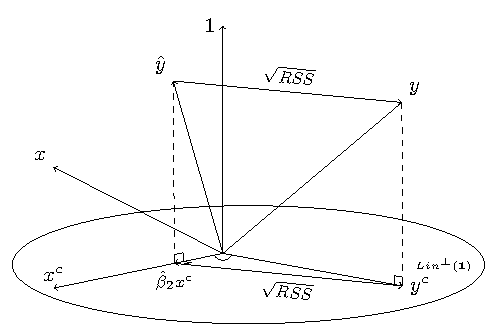
\includegraphics[width=0.45\linewidth]{figures/04_ttest.pdf}
\label{fig:ttest_3d}}
%\hspace{4ex}
\subfigure[]{
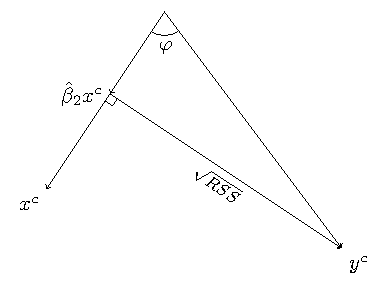
\includegraphics[width=0.45\linewidth]{figures/04_ttest_lin.pdf}
\label{fig:ttest_lin}}
\caption{\subref{fig:pcorr_t_x}: Regression of $y$ onto $Lin(x, \mathbf{1})$ and appropriate projections;
\subref{fig:pcorr_t_y}: $Lin^{\perp}(\mathbf{1})$.}
\end{center}
\end{figure}

\subsection{F-distribution}

\subsection{F-test}

The significance of several coefficients at once can be tested with the F-test.
The F-statistic has the following form
\[
F = \frac{(RSS_{R} - RSS_{UR})/q}{RSS_{UR}/(n-k_{UR})}
\]
where indices $R$ and $UR$ stand for the restricted and unrestricted models
respectively, $n$ — number of observations, $k$ — number of regressors,
$q$ — number of equtions used in the null hypothesis.

Due to plotting limitations, we consider the unrestricted model to be
\[
y = \beta_1 + \beta_2 x + u
\]
and the restricted model to be
\[
y = \alpha_1 + v
\]
Note that there was a choice in the restricted models.

We perform both regressions in order to get the ressiduals and plot them
in Figure~\ref{fig:ftest}.
Adjusted to the degrees of freedom, the ratio can be expressed in terms of the
angle between two vectors, $\varphi$, as demonstrated in Figure~\ref{fig:ftest}
\[
F = \frac{(RSS_{R} - RSS_{UR})/q}{RSS_{UR}/(n-k_{UR})} = \ctg^2 \varphi
\]

\begin{figure}
\centering
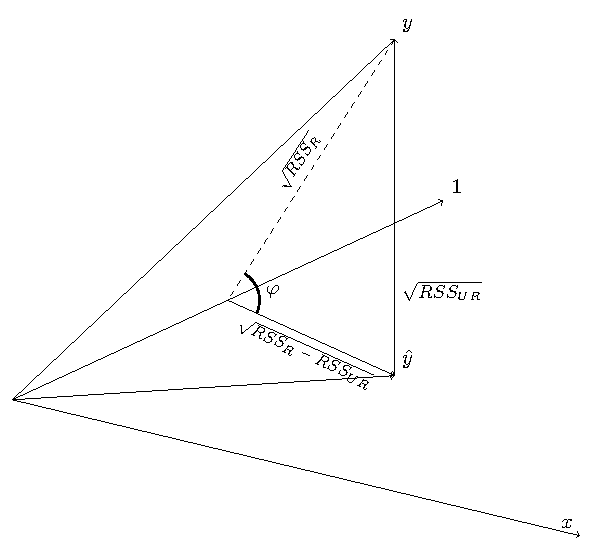
\includegraphics[width=0.55\linewidth]{figures/04_ftest.pdf}
\caption{F-statistic as the cotangens squared of $\varphi$}
\label{fig:ftest}
\end{figure}
